\url{http://tex.stackexchange.com}.

\LaTeX. 

%% Some commands which make the plotting work properly from inkscape.
%% Align bottom of text to node 
\newcommand{\ISb}[1]{\makebox[0pt]{{#1}}} 
%% Align centre of text to node 
\newcommand{\ISc}[1]{\makebox[0pt]{\raisebox{-0.5\height}{#1}}}
%% Align top of text to node 
\newcommand{\ISt}[1]{\makebox[0pt]{\raisebox{-\height}{#1}}}
%% Align y-axis ticklabels
\newcommand{\yticks}[1]{\makebox[0pt][r]{\raisebox{-0.5\height}{#1}\hspace*{1.8mm}}}
\newcommand{\ylabel}[1]{\makebox[0pt][r]{\raisebox{-0.5\height}{#1}\hspace*{6.7mm}}}
%% Align x-axis ticklabels
\newcommand{\xticks}[1]{\makebox[0pt][c]{\raisebox{-3.8mm}{#1}}}
\newcommand{\xlabel}[1]{\makebox[0pt][c]{\raisebox{-7.0mm}{#1}}}
%% Align colorbar ticklabels
\newcommand{\lticks}[1]{\makebox[0pt][l]{\hspace*{2.0mm}\raisebox{-0.5\height}{#1}}}

%% Align colorbar ticklabels
\newcommand{\sftl}[1]{\makebox[0pt][l]{\hspace*{0.8mm}\raisebox{-3.2mm}{#1}}} %% Top left
\newcommand{\sftr}[1]{\makebox[0pt][l]{\hspace*{-6.0mm}\raisebox{-3.2mm}{#1}}} %% Top right


\verb|savequote| 

\mccorrect{like this one}

\begin{mccorrection}
For larger chunks, like this paragraph or indeed entire figures, you can use the \verb|mccorrection| environment.  This environment highlights paragraph-sized and larger blocks with the same blue colour.
\end{mccorrection}

\begin{figure}
\centering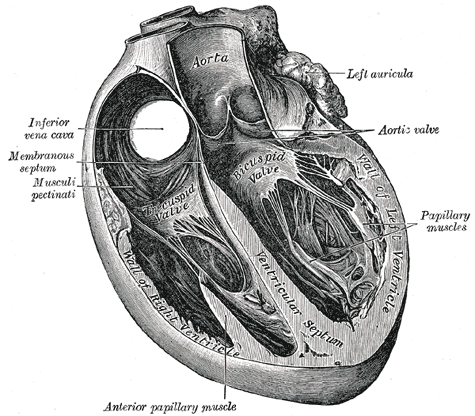
\includegraphics[width=0.7\textwidth]{figures/sample/Gray498.png} 
\caption[Four-chamber illustration of the human heart.]{Four-chamber illustration of the human heart.  Clockwise from upper-left: right atrium, left atrium, left ventricle, right ventricle.}
\label{fig:fourchamber}
\end{figure}

\subsection{Diagnostic Imaging}
\label{sub:diagnostic}
